% !TEX TS-program = xelatex
% !TEX encoding = UTF-8 Unicode
\documentclass[AutoFakeBold]{MyFormat}

\usepackage{listings, cite}
\usepackage{hyperref}


\hypersetup{
    hidelinks,                          % 暂时没看出有啥用
    colorlinks=true,                    % 是否要上色,不加这一行就没效果
    % allcolors=blue,                   % 图个省事全都一个色
    pdfstartview=Fit,                   % 不太懂
    breaklinks=true,                    % 允许链接断行
    urlcolor=blue,                      % url链接的颜色
    anchorcolor=green,                  % 锚文本的颜色
    citecolor=red,                      % 引用的颜色
    linkcolor=black,                    % 例如目录这种超链接的颜色
}

% \CTEXsetup[format+={\color{red}}]{section}

\lstset{
 columns=fixed,       
 numbers=left,                                        % 在左侧显示行号
 numberstyle=\tiny\color{gray},                       % 设定行号格式
 frame=none,                                          % 不显示背景边框
 backgroundcolor=\color[RGB]{245,245,244},            % 设定背景颜色
 keywordstyle=\color[RGB]{40,40,255},                 % 设定关键字颜色
 numberstyle=\footnotesize\color{darkgray},           
 commentstyle=\it\color[RGB]{0,96,96},                % 设置代码注释的格式
 stringstyle=\rmfamily\slshape\color[RGB]{128,0,0},   % 设置字符串格式
 showstringspaces=false,                              % 不显示字符串中的空格
 language=python,                                        % 设置语言
}

\begin{document}
%=====%
%
%封皮页填写内容
%
%=====%

% 标题样式 使用 \title{{}}; 使用时必须保证至少两个外侧括号
%  如: 短标题 \title{{第一行}},  
% 	      长标题 \title{{第一行}{第二行}}
%             超长标题\tiitle{{第一行}{...}{第N行}}

\title{{2022.07.31学习笔记}}
\entitle{{论文复现及学习笔记}}
\author{Sillin Ini\\Pinyi Huang}
\maketitle
\thispagestyle{empty}
\newpage

%生成目录
\tableofcontents
\thispagestyle{empty}
\newpage

%文章主体
\mainmatter




% =======正文从第一章开始
\setcounter{chapter}{0}
\chapter{问题整理与记录}


\chapter{OpenCV函数学习记录}
\section{关于每个image的知识}
\par 通过\textit{cv2.imread}读取的每个image都是一个np.array数组。
\par 通常其形状为\textit{(height, width, 3)},一定要注意height位于width之前。


\section{关于\textit{cv2.circle}函数}
\par cv2.circle(img, center, radius, color, thickness)
\par 其中,一定要注意,center接收的坐标为(width, height),这与一般的坐标是反过来的。

\section{列表元素相加减}
\par 列表对应元素相加减,可以使用zip函数进行。如a和b是两个同形状列表:
\par result = [i - j for i, j in zip(a, b)]


\chapter{论文阅读及思考记录}
\par 以下为阅读过的论文,及其主要贡献的个人思考和总结。

\section{\textit{Short and Long Range Relation
Based Spatio-Temporal Transformer for
Micro Expression Recognition(2021.12)}\cite{zhang2021short}}

\subsection{论文的主要贡献和主要思想}
\par 个人总结,这篇论文的主要贡献和主要思想如下:
\begin{enumerate}
    \item 将视频中每一帧与微表情起始帧计算光流场,而非任意两连续帧。\\
    计算相邻帧之间的光流场时,在前半部分有相似的光流,后半部分则强度相似,方向相反。\\
    而用这里提出的方法,发现光流场总是沿同样的方向,只是前半部分的强度逐渐递增,
    后半部分的强度逐渐递减。这导致了与每个微表情相关的更稳定和可区别的特征。
    \item \textbf{\Large \underline{首个}}完全摒弃CNN进行特征提取的MER神经网络模型。
    其认为,CNN只能在固定窗口大小中进行短期空间特则提取,由此无法学习到同样十分重要的长期空间特征。
    而Encoder of Transformer中使用到的Multi-head Self-attention Mechanism(MSM)自注意力
    机制,可以很好的学习到短期和长期空间特征,由此其完全摒弃了CNN的使用。
    \item 时间聚合:使用了LSTM Aggregator进行聚合,并与Mean Aggregator进行了对比。聚合函数确保了Transformer模型可以被训练并应用于每一帧的空间特征集,然后处理每个样本中各帧之间的时间关系。
\end{enumerate}


\subsection{数据预处理阶段}
\par 首先是\underline{人脸图像裁剪阶段}:其在表情峰值顶点帧提取人脸68个特征点,然后根据公式计算人脸的大小,并以第30号点为中心(标号以0开始),截取一帧中的这一部分图像。由此可以保证几乎整张人脸都被囊括在这个裁剪的图像内部。
\begin{equation}
    s = (y_{apex[8]} - y_{apex[19]}) + (y_{apex[8]} - y_{apex[57]})
\end{equation}
\par 其中,s表示截取图像的长和宽;y轴表示的是图像的height轴,注意在图像当中,height轴向下为正方向。
\par 接下来是\underline{时空插值阶段}:其在原始视频中应用了帧插值方法,有效地进行了数据增强。
\par 与简单的线性插值不同,这里提出了一种新的插值方法,这种方法在光流方面更平滑。这里使用了RIFE(\textit{Real-time Intermediate Flow Estimation})方法\upcite{huang2020rife},这是一个端到端的可训练神经网络,它能很快和直接的估计中间光流。
\par 传统的RIFE在连续的两帧之间进行插值,得到一个中间帧。而本文中,通过递归插值的方法获取多个中间帧。具体的说,操作步骤如下:
\begin{itemize}
    \item 首先以连续的两帧$I_0, I_1$作为输入,得到一个中间帧$\hat{I}_{0.5}$,即t=0.5时刻的帧;
    \item 其次递归使用RIFE,对$I_0$和$\hat{I}_{0.5}$进行插值,得到$\hat{I}_{0.25}$。如此反复;
    \item 另外有一点,本文中优先对顶点帧附近进行插值,最后得到的插值队列可以被表示为:$\{\hat{I}_{a-0.5},\hat{I}_{a+0.5},\hat{I}_{a-1.5},\hat{I}_{a+1.5},...,\hat{I}_{o+0.5} \  or \  \hat{I}_{f-0.5}\}$,这里的$a, o, f$分别表示顶点帧、起始帧(onset frame)和偏移帧(offset frame)。
\end{itemize}
\par 值得注意的是,在CASME II和SAMM数据库中,顶点帧的位置已经被明确指出了;而在SMIC-HS数据库中则没有。因此采用了SMIC-HS的中间帧作为该样本的顶点帧。



\subsection{ViT(\textit{Vision Transformer})的应用}
\par 神经网络初期使用了一个ViT结构,该结构的示意图如下所示。
\begin{figure}[!h]
    \centering
    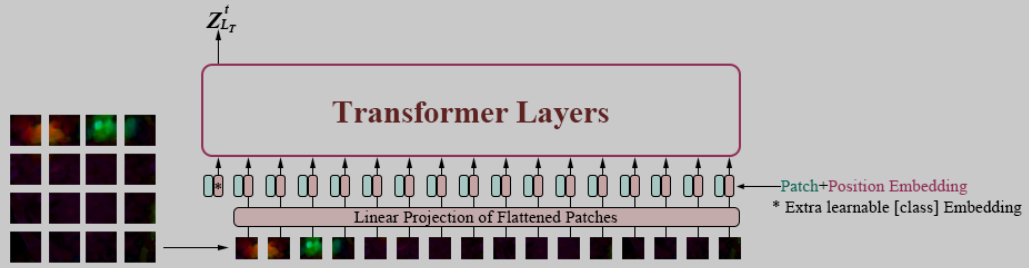
\includegraphics[width=\linewidth]{figures/2022.07.31/ViT.png}
    \caption{ViT模型结构示意图}
\end{figure}
\par 对模型的理解:
\par 由于Transformer是用于NLP任务的结构,其输入需要是一个词结构。而对于MER来说,其输入通常是一个
视频(并从中提取每一帧),由此便需要将图像转换为词结构。这里使用到的方法是将图片分割成若干个小块
patch,这里的每个小块就相当于句子里的每个词。而\textit{Patch Embedding}就是把每个patch经过一个
全连接网络压缩成一定维度的向量,即词向量。
\par 而这里的词嵌入过程,就是图中的\textit{Linear Projection of Flattened Patches}部分。
\par 具体来说,就是使用了一个kernel\_size = stride = patch\_size的nn.Conv2d进行压缩,并且
in\_channels = C,图像通道数(一般为RGB图像,即C = 3),out\_channels = embed\_dim,即词向量的
维度。
\par 此外,为了表示每个patch的位置信息(即每个词在句子中的位置信息),还需要加入一个\textit{Position
Embedding}位置嵌入。此处使用到的位置信息通常是\underline{可训练的位置信息},参数通过训练来进行调整
(具体怎么实现暂时还未了解,似乎是一个nn.Embedding模块)。
\par 同时,ViT添加了一个cls\_token(\textit{classification token}),可以这样理解:
其他的embedding表达的都是不同的patch的特征,而cls\_token是要综合所有patch的信息,
产生一个新的embedding,来表达整个图的信息。这个token也是可学习的。
\\\hspace*{\fill}
\par 并且,这里的Encoder of Transformer过程与传统的Encoder略有不同,其结构图对比如下所示。
\begin{figure}[htbp]
    \centering
    \begin{minipage}[t]{0.4\linewidth}
        \centering
        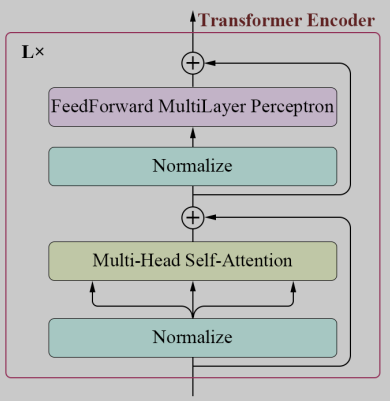
\includegraphics[width=\textwidth]{figures/2022.07.31/ViT_Encoder.png}
        \centerline{(a) Encoder of ViT}
    \end{minipage}
    \begin{minipage}[t]{0.4\linewidth}
        \centering
        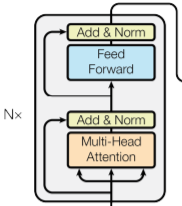
\includegraphics[width=\textwidth]{figures/2022.07.31/original_Encoder.png}
        \centerline{(b) Encoder of original Transformer}
    \end{minipage}
    \caption{两种不同的Encoder结构的对比}
\end{figure}
\par 由上图可以发现,两者关于归一化操作和MSM、FFN(\textit{Feed-Forward Network})的顺序恰好相反。
\\\hspace*{\fill}
\par 并且,ViT中使用\textbf{\Large \underline{DropPath代替了传统的Dropout}},
其主要效果是其效果是将深度学习模型中的多分支结构的子路径随机“删除”,可以防止过拟合,提升模型表现,
而且克服了网络退化问题。
\par 在向前传播的时候,让神经元以一定概率停止工作。这样可以使模型泛化能力变强,
因为神经元会以一定概率失效,这样的机制会使结果不会过分依赖于个别神经元。
训练阶段,以keep\_prob概率使神经元失效,而推理的时候,会保留所有神经元的有效性,
因此,训练时候加了dropout的神经元推理出来的结果要除以keep\_prob。
\par 在Dropout中也有同样的体现:未被置零的元素需要除以(1 - dropout),由此来保证整体的期望在Dropout
前后不会发生变化。
\par 两者的主要区别有:
\begin{enumerate}
    \item Dropout是以一定比例,将某个向量内部的元素置为0;
    \item DropPath是以一定的概率,将神经网络中的一条路径“删除”。
\end{enumerate}
\par 在传统的Transformer结构论文代码\upcite{lei2021FGRMER}重写中,我自己曾写过其中的Dropout代码,
其都是使用nn.Dropout(dropout=0.5)来创建的。而相对应的,ViT中的dropout位置相同,而其需要改成使用
DropPath进行使用即可。
\par 有一点很奇怪,有两个不同的github仓库,均对ViT模型进行了实现,且均使用PyTorch进行编写。
但两者实现Dropout的方式不相同,
\href{https://github.com/lucidrains/vit-pytorch#vision-transformer---pytorch}{其一}
直接使用nn.Dropout,而
\href{https://github.com/rwightman/pytorch-image-models/blob/master/timm/models/vision_transformer.py}
{另外一个}则使用了DropPath的方式。
\par 而
\href{https://github.com/google-research/vision_transformer/blob/main/vit\_jax/models\_vit.py}
{官方实现}中则是使用了nn.Dropout版本。这是否意味着两种方式均可实现,而从实际效果来说没有较大区别?

\subsection{\textit{Temporal Aggregation}时空聚合}
\par 时空聚合中使用了LSTM Aggregator进行聚合操作,并将其与Mean Aggregator进行了对比。对比后发现LSTM Aggregator的效果好于Mean Aggregator。其具体的使用步骤如下,以一层LSTM Aggregator为例。
\begin{figure}[!h]
    \centering
    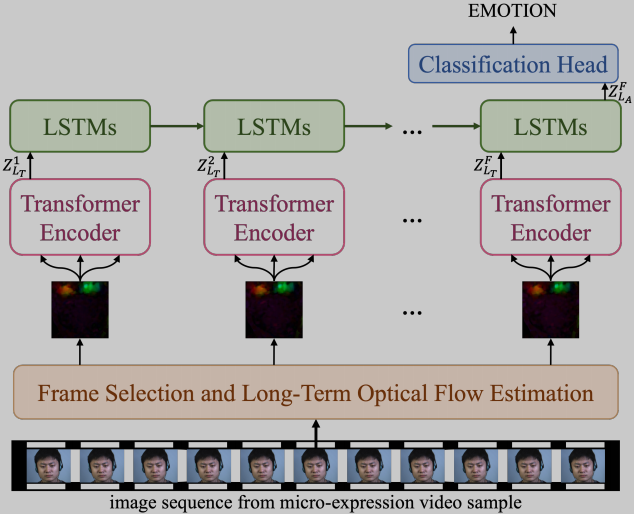
\includegraphics[width=0.6\linewidth]{figures/2022.07.31/SLSTT model.png}
    \caption{这里指应该是画的只有一层LSTM Aggregator的情况}
\end{figure}
\par 这里的时空聚合的输入是每一帧经过一系列操作后,由Encoder输出的结果,即一个视频的帧数即为LSTM迭代的次数。图中画出了一系列的LSTMs,实际上就只是一个LSTM层被数次迭代。
\par 而最后的输出$Z^F_{L_A}$的含义是,经过了$F$帧数和$L_A$个层数。这里的$L_A$表示$L_T + L_{LSTM}$,其中$L_T$表示Transformer的总层数,$L_{LSTM}$表示LSTM Aggregator的总层数。
\par 聚合函数确保了文中的Transformer模型可以被训练和应用于每一帧的空间特征集,然后处理每个样本中的帧之间的时间关系。由于LSTM可以学习时间关系,因此帧间的时序关系就被学习了。
\par 并且很重要的一点是,与其他通过改变视频帧顺序,来增强数据库的方法不同,这里的聚合并没有改变微表情视频样本的时序关系。





\bibliography{bib/literatures}
\bibliographystyle{ieeetr}
\end{document}